%%
%% Copyright (C) Hochschule Esslingen, 2011
%%
%% $Id: example.tex 131 2011-10-16 01:11:22Z uwe $
%%
%% This work may be distributed and/or modified under the
%% conditions of the LaTeX Project Public License, either version 1.3
%% of this license or (at your option) any later version.
%% The latest version of this license is in
%%   http://www.latex-project.org/lppl.txt
%% and version 1.3 or later is part of all distributions of LaTeX
%% version 2005/12/01 or later.

\makeglossaries

\begin{document}

% If you wish to uncover everything in a step-wise fashion, uncomment
% the following command: 
% \beamerdefaultoverlayspecification{<+->}

\mode<article>{\maketitle}

\begin{frame}
  \titlepage
\end{frame}

\ifoverview
% ----- No TOC in course overview
\else
\begin{frame}{Content}
  \tableofcontents
\end{frame}
\fi

\ifoverview
\section{Introduction: Chapter 1: Distributed Real-Time Systems}


Lecturer: Vikas Agrawal, vikas.agrawal@hs-esslingen.de,
Room F 01.301

\section{Literature for this lecture}\label{literature-for-this-lecture}

\begin{longtable}[c]{@{}l@{}}
\toprule
\textbf{Text books for this lecture}\tabularnewline
{[}1.1{]}Kopetz, H.: Distributed Real-Time Systems, Springer 2008\tabularnewline
{[}1.2{]}Buttazzo, G.: Hard Real-Time Computing Systems, Springer 2005\tabularnewline
\bottomrule
\end{longtable}

\begin{longtable}[c]{@{}l@{}}
\toprule
\textbf{Complementing texts}

\emph{Some books complementing the material treated in this lecture}\tabularnewline
{[}2.1{]}Liu, J.S.: Real-Time Systems, Prentice Hall 2000\tabularnewline
{[}2.2{]}Vérissimo, P; Rodrigues, L.: Distributed Systems for System Architects, Kluwer 2001\tabularnewline
{[}2.3{]}Laplante, P.: Real-Time Systems Design and Analysis, IEEE Press, 2004\tabularnewline
{[}2.4{]}Halbwachs, N.: Synchronous Programming of Reactive Systems, Kluwer 1993\tabularnewline
{[}2.5{]}Zimmermann, W.; Schmidgall, R.: Bussysteme in der Fahrzeugtechnik, Vieweg 2006 (German only)\tabularnewline
\bottomrule
\end{longtable}

\begin{longtable}[c]{@{}l@{}}
\toprule
\textbf{Journal Articles and Web Documents}

\emph{Original journal articles and documents from the web pertaining to this lecture}\tabularnewline
{[}3.0{]}Albert, A.:Comparison of Event-Triggered and Time-Triggered Concepts with Regard to Distributed Control Systems, Embedded World, 2004, Nürnberg\tabularnewline
%http://www.semiconductors.bosch.de/pdf/embedded_world_04_albert.pdf
{[}3.1{]}Müller, B.; Führer, T.; Hartwich, F.; Hugel, R.; Weiler, H.: Fault Tolerant TTCAN Networks, Proceedings 8th International CAN Conference; 2002; Las Vegas, NV\tabularnewline
%http://www.semiconductors.bosch.de/pdf/Fault_Tolerant_TTCAN.pdf\tabularnewline
\bottomrule
\end{longtable}

\begin{frame}{Introduction}{Part 1}
    \begin{block}{Overview}
Chapter 1	  The Real-Time Environment\\
Chapter 2	  Distributed Real-Time Systems\\
Chapter 3	  Global Time\\
Chapter 4	  Modeling Real-Time Systems\\
Chapter 5	  Real-Time Entities and Images\\
Chapter 6	  Fault Tolerance\\
Chapter 7	  Real-Time Communication\\
Chapter 8	  Time-Triggered Protocols\\
Chapter 9	  Input and Output\\
Chapter 10	Real-Time Operating Systems: OSEK and AUTOSAR\\
Chapter 11	Real-Time Scheduling\\
Chapter 12	Validation
\end{block}
\end{frame}


\begin{frame}{Introduction}{Part 1}
    \begin{block}{The Real-Time Environment}
\begin{itemize}
\item
  Definition of a real-time system.
\item
  Simple model with operator, computer system, and controlled object.
\item
  Introduction of distributed real-time systems.
\item
  Hard real-time systems and soft real-time systems.
\item
  Functional, temporal, and dependability requirements.
\item
  Sphere of control
\item
  Event-triggered versus time-triggered systems.
\end{itemize}
\end{block}
\end{frame}

\begin{frame}{Introduction}{Part 2}
    \begin{block}{Distributed Real-Time Systems}
\begin{itemize}
\item
  Distributed system architecture overview, clusters, nodes,
  communication network
\item
  Structure of node with host computer, communication network interface,
  communication controller
\item
  Event and state messages, gateways.
\item
  Concept of composability.
\item
  Event- and time-triggered communication systems.
\item
  Scalability, dependability, issues of physical installation.
\end{itemize}
\end{block}
\end{frame}


\begin{frame}{Introduction}{Part 3}
    \begin{block}{Global Time}
\begin{itemize}
\item
  Notions of causal order, temporal order, and delivery order
\item
  External observers, reference clocks, and global time base
\item
  Sparse time base to view event order in a distributed real-time system
\item
  Internal clock synchronization to compensate for drift offset.
  Influence of the communication system jitter on the precision of the
  global time base.
\item
  External time synchronization, time gateways, and the Internet network
  time protocol (NTP)
\end{itemize}
\end{block}
\end{frame}


\begin{frame}{Introduction}{Part 4}
    \begin{block}{Modeling Real-Time Systems}
\begin{itemize}
\item
  Introduction of a conceptual model for real-time systems
\item
  Tasks, nodes, fault-tolerant units, clusters
\item
  Simple and complex tasks
\item
  Interface placement and interface layout
\item
  Temporal control and logical control
\item
  The history state
\end{itemize}
\end{block}
\end{frame}


\begin{frame}{Introduction}{Part 5}
    \begin{block}{Real-Time Entities and Images}
\begin{itemize}
\item
  Real-time entities
\item
  Observations, state and event observations
\item
  Real-time images as current picture of real-time entity, and real-time
  objects
\item
  Temporal accuracy and state estimation to improve real-time image
  accuracy
\item
  Permanence in case of race conditions and idempotency with replicated
  messages
\item
  Replica determinism to implement fault-tolerance by active redundancy
\end{itemize}
\end{block}
\end{frame}


\begin{frame}{Introduction}{Part 6}
    \begin{block}{Fault Tolerance}
\begin{itemize}
\item
  Failures, Errors, and Faults
\item
  Error Detection
\item
  A Node as a Unit of Failure
\item
  Fault Tolerant Units
\item
  Reintegration of a Repaired Node
\item
  Design Diversity
\end{itemize}
\end{block}
\end{frame}


\begin{frame}{Introduction}{Part 7}
    \begin{block}{Real-Time Communication}
\begin{itemize}
\item
  Real-Time Communication Requirements
\item
  Flow Control
\item
  OSI Protocols for Real-Time
\item
  Fundamental Conflicts in Protocol Design
\item
  Media-Access Protocols
\item
  Performance Comparison: ET versus TT
\item
  The Physical Layer
\end{itemize}
\end{block}
\end{frame}


\begin{frame}{Introduction}{Part 8}
    \begin{block}{Time-Triggered Protocols}
\begin{itemize}
\item
  Introduction to Time-Triggered Protocols
\item
  Overview of the TTP/C Protocol Layers
\item
  The Basic CNI
\item
  Internal Operation of TTP/C
\item
  TTP/A for Field Bus Applications
\end{itemize}
\end{block}
\end{frame}


\begin{frame}{Introduction}{Part 9}
    \begin{block}{Input and Output}
\begin{itemize}
\item
  The dual role of time
\item
  Agreement protocol
\item
  Sampling and polling
\item
  Interrupts
\item
  Sensors and actuators
\item
  Physical installation
\end{itemize}
\end{block}
\end{frame}


\begin{frame}{Introduction}{Part 10}
    \begin{block}{Real-Time Operating Systems: OSEK and AUTOSAR}
\begin{itemize}
\item
  Task management
\item
  Interprocess communication
\item
  Time management
\item
  Error detection
\item
  OSEK and AUTOSAR
\end{itemize}
\end{block}
\end{frame}


\begin{frame}{Introduction}{Part 11}
    \begin{block}{Real-Time Scheduling}
\begin{itemize}
\item
  The scheduling problem
\item
  The adversary problem
\item
  Dynamic scheduling, dynamic priority servers
\item
  Static scheduling, fixed priority servers
\end{itemize}
\end{block}
\end{frame}


\begin{frame}{Introduction}{Part 12}
    \begin{block}{Validation}
\begin{itemize}
\item
  Building a Convincing Safety Case
\item
  Formal Methods
\item
  Testing
\item
  Fault Injection
\item
  Dependability Analysis
\end{itemize}
\end{block}
\end{frame}

\fi

\ifpartI
%
%      Introduction into UML, Principles of Object Oriented Design
%
\section{Part \partNo\ Learning Objectives}

\begin{frame}{What are you about to learn?}
   \begin{block}{Knowledge}
       \begin{itemize}
           \item What is architecture?
           \item Architectural objectives in software design
           \item UML structural modeling elements 
   \end{itemize}
   \end{block}
   \begin{block}{Skills}
       \begin{itemize}
           \item Can detect violations of object oriented design principles
           \item Can explain all object oriented design principles using UML diagrams
   \end{itemize}
\end{block}
\end{frame}

%-------------------------------------------------------------------
\section{What is Architecture?}

\begin{frame}[fragile]{The Parthenon in Athens, Greece}
\begin{center}
  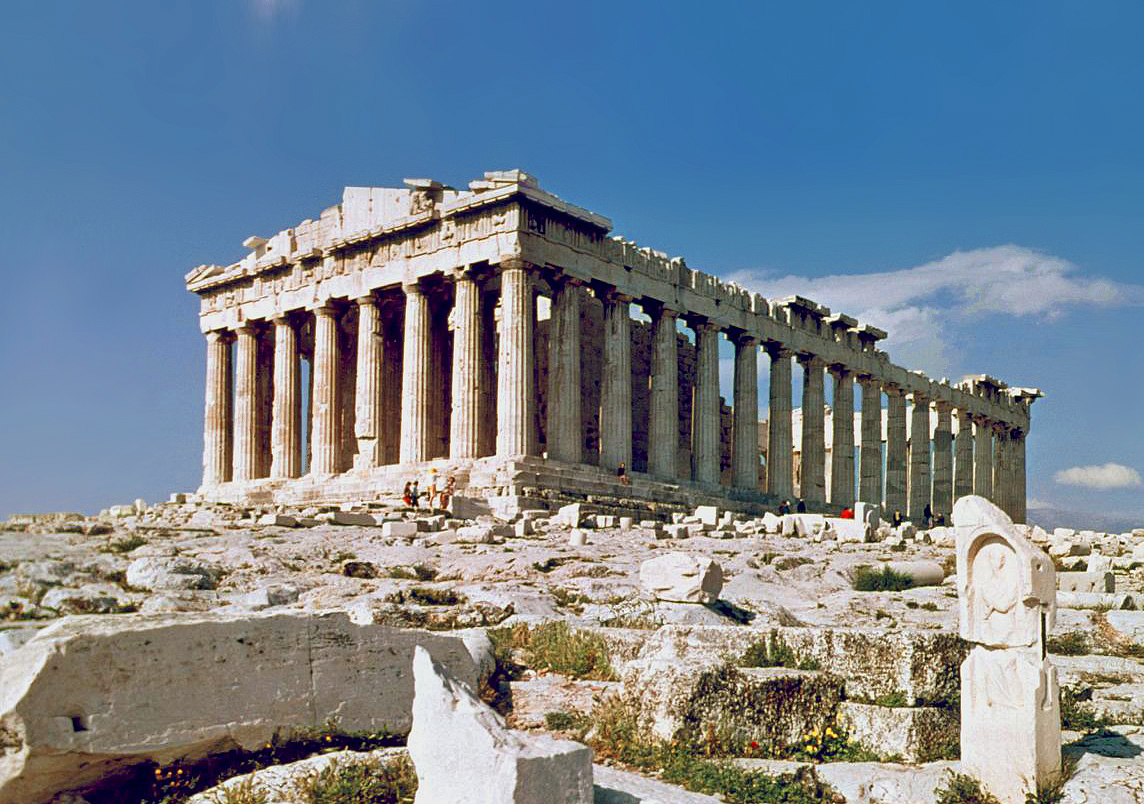
\includegraphics[height=180pt]{partenon.jpg}
\end{center}
\end{frame}

\begin{frame}[fragile]{Some Genius Improvising}
\begin{center}
  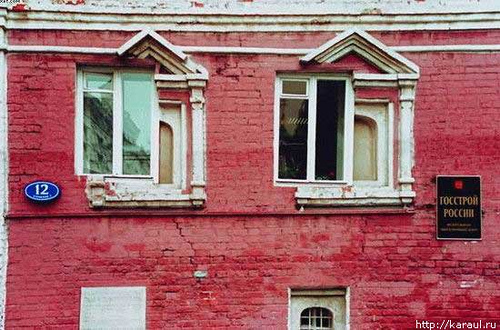
\includegraphics[height=180pt]{badbuilding1.jpg}
\end{center}
\end{frame}

\begin{frame}[fragile]{The Houses of Parliament, London}
\begin{center}
  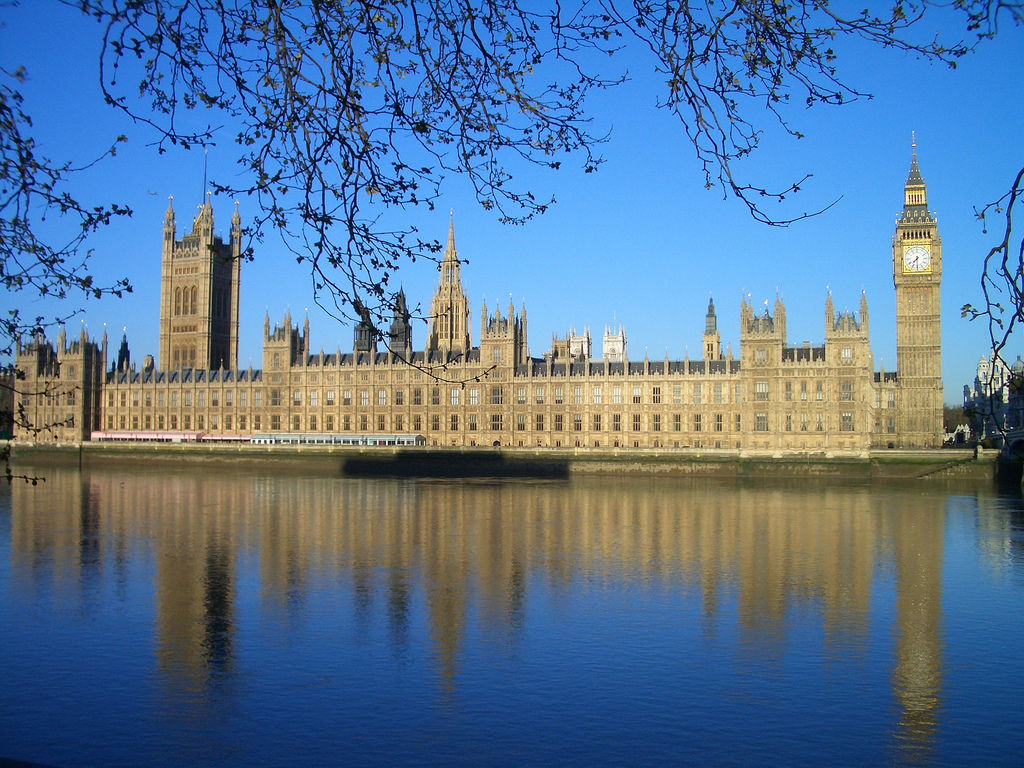
\includegraphics[height=180pt]{Westminster.jpg}
\end{center}
\end{frame}

\begin{frame}[fragile]{The Bauhaus in Dessau, Germany}
\begin{center}
  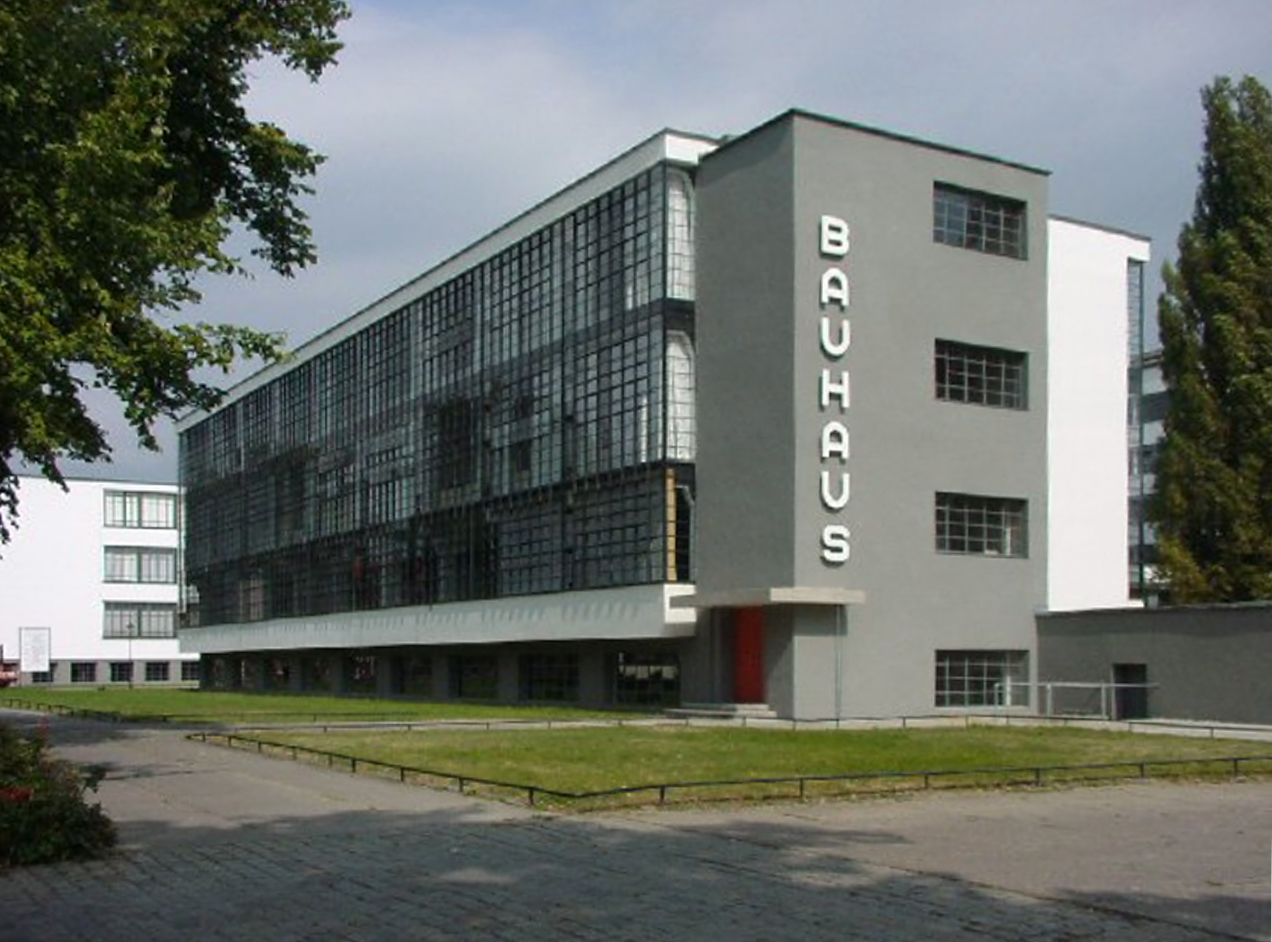
\includegraphics[height=180pt]{Bauhaus.jpg}
\end{center}
\end{frame}

\begin{frame}[fragile]{The Taj Mahal, India}
\begin{center}
  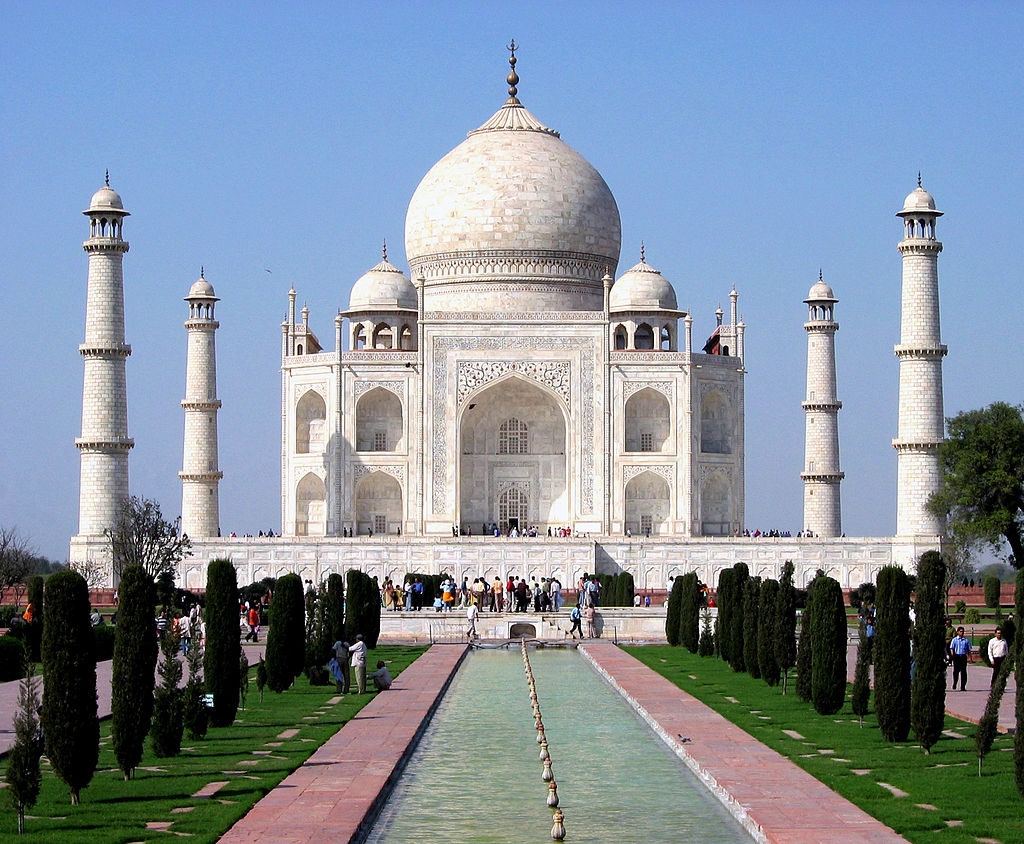
\includegraphics[height=180pt]{TajMahal.jpg}
\end{center}
\end{frame}

\begin{frame}[fragile]{The National Congress of Brazil}
\begin{center}
  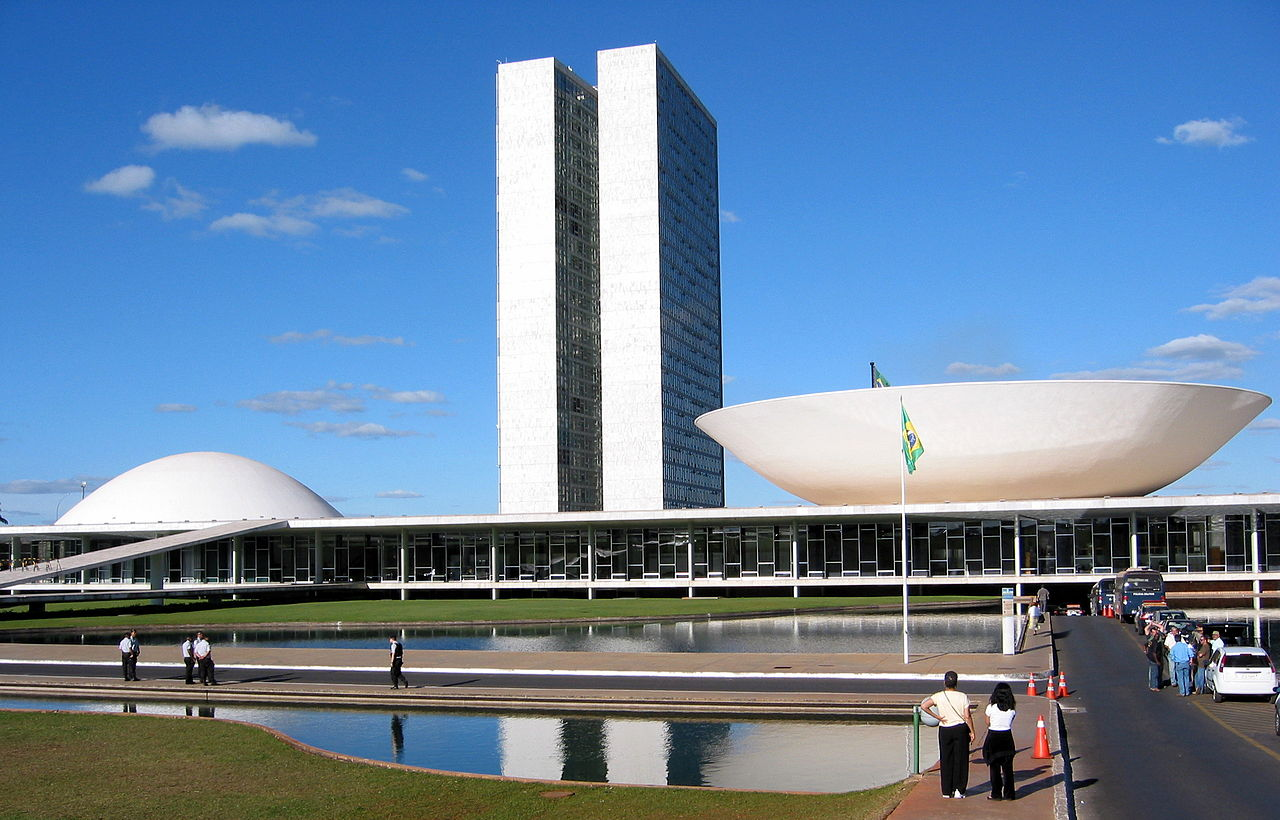
\includegraphics[height=180pt]{CongressoDoBrasil.jpg}
\end{center}
\end{frame}

\begin{frame}[fragile]{The Carpenter did the Design}
\begin{center}
  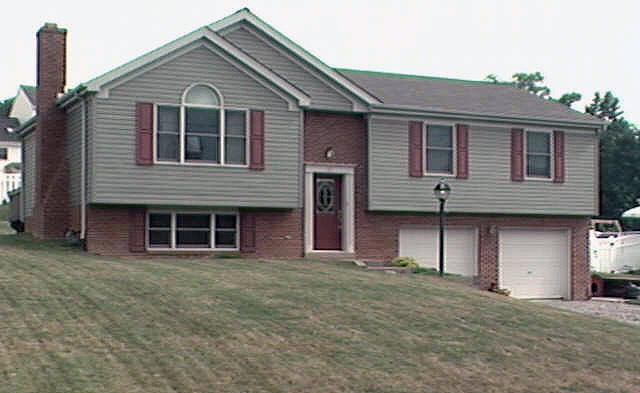
\includegraphics[height=180pt]{badbuilding2.jpg}
\end{center}
\end{frame}

\begin{frame}[fragile]{The Gare de Oriente in Lisbon, Portugal}
\begin{center}
  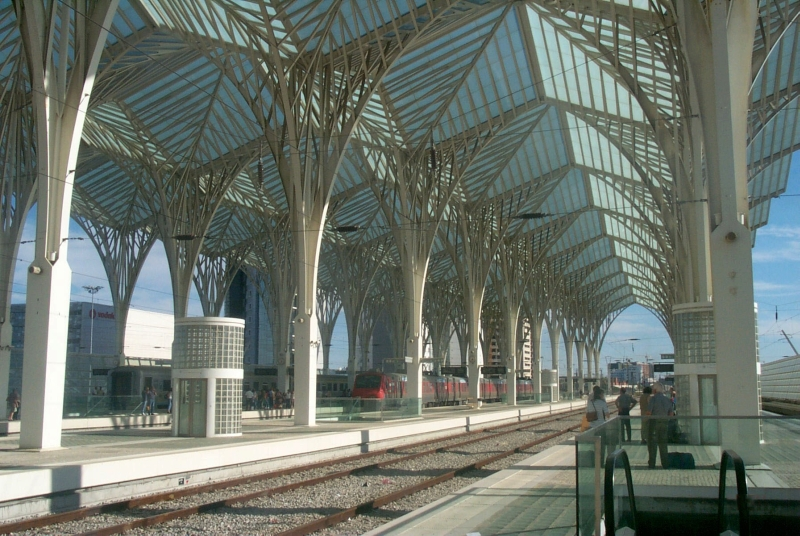
\includegraphics[height=180pt]{OrienteStationLisboa.jpg}
\end{center}
\end{frame}

\begin{frame}[fragile]{The Golden Pavilion in Kyoto, Japan}
\begin{center}
  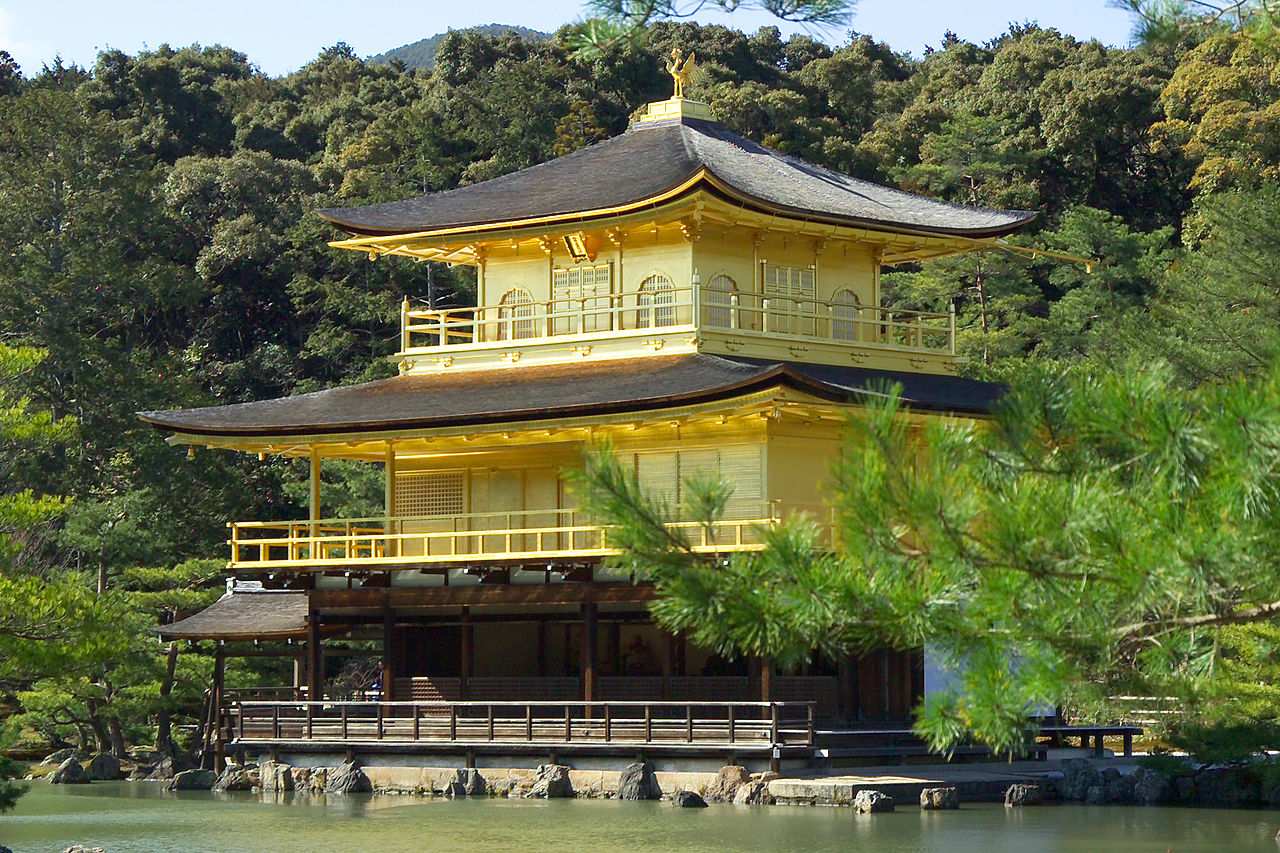
\includegraphics[height=180pt]{Kinkaku.jpg}
\end{center}
\end{frame}

\begin{frame}[fragile]{Notre Dame de Paris, France}
\begin{center}
  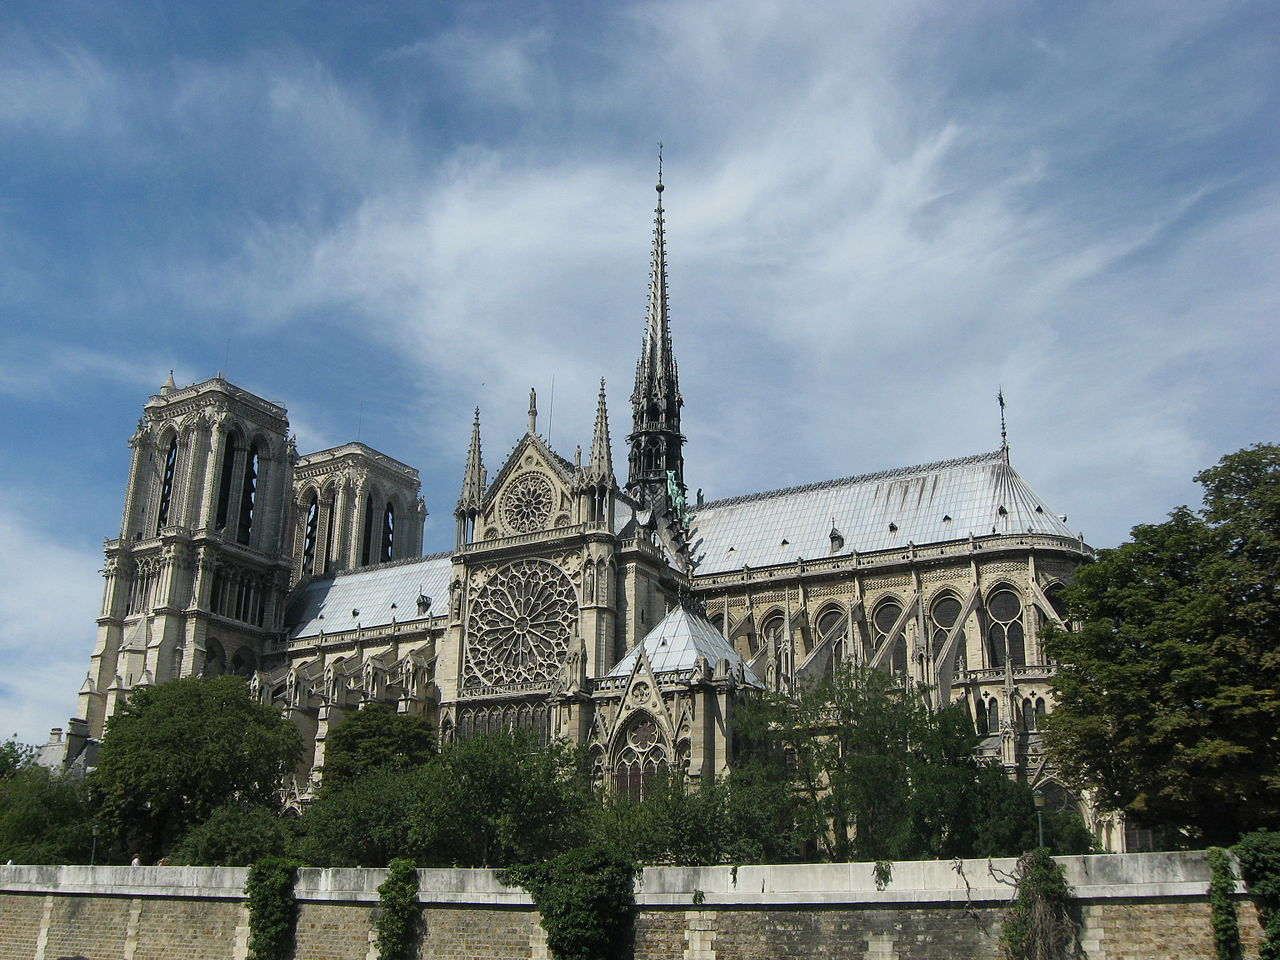
\includegraphics[height=180pt]{NotredameParis.jpg}
\end{center}
\end{frame}

\begin{frame}[fragile]{MI6 Headquarter in London}
\begin{center}
  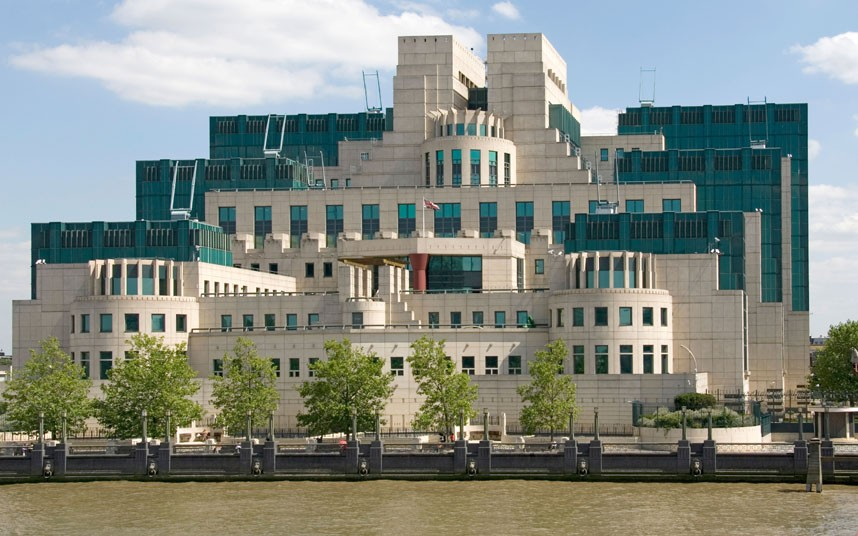
\includegraphics[height=180pt]{mi6.jpg}
\end{center}
\end{frame}

\begin{frame}[fragile]{Shantytown, New Orleans}
\begin{center}
  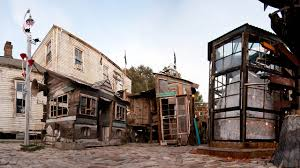
\includegraphics[height=180pt]{badbuilding3.jpg}
\end{center}
\end{frame}

\begin{frame}[fragile]{The Opera House in Sydney, Australia}
\begin{center}
  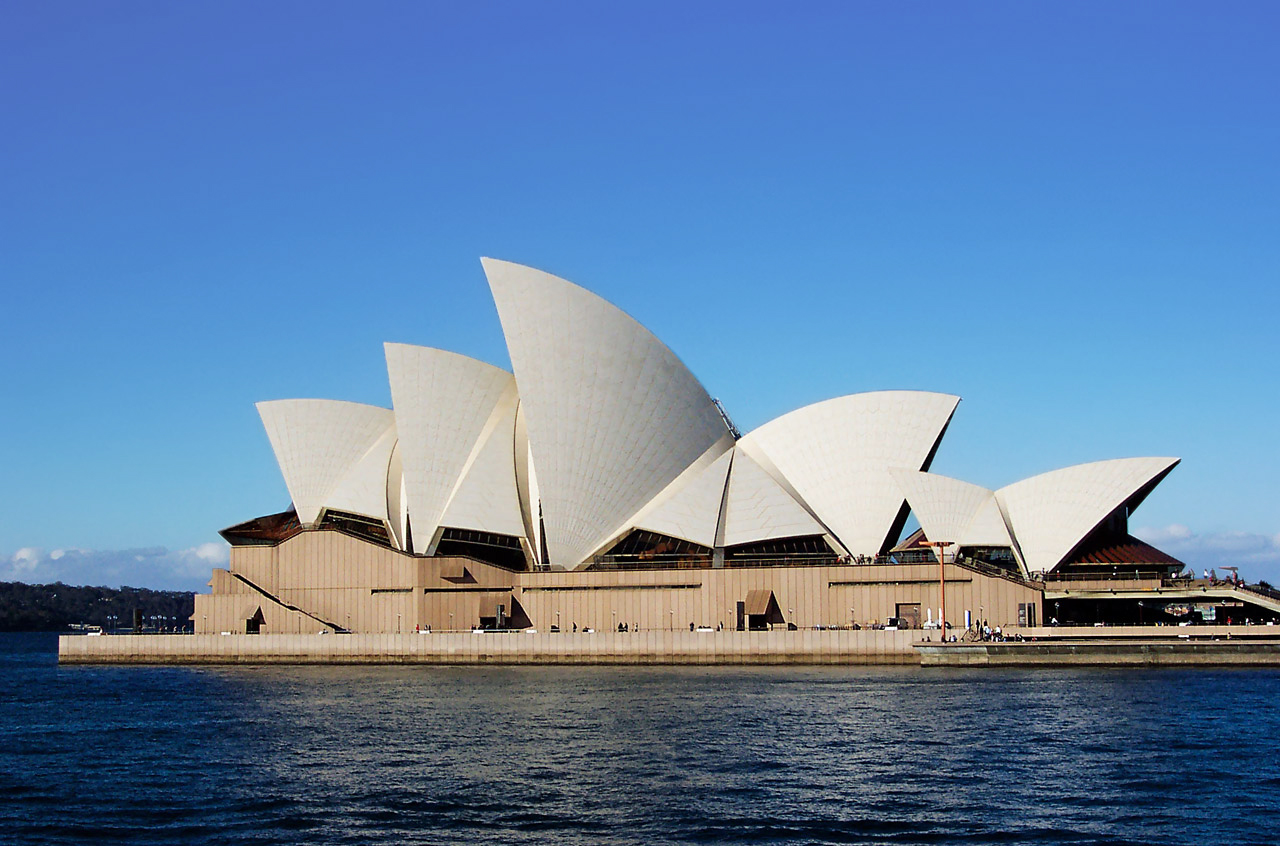
\includegraphics[height=180pt]{SydneyOpera.jpg}
\end{center}
\end{frame}

\begin{frame}{What is Architecture?}
   \begin{block}{Architecture}
       \begin{itemize}
           \item A general term to describe buildings and other physical and some non-physical structures.
           \item The art and science of designing buildings and (some) nonbuilding structures ("Baukunst").
           \item The style of design and method of construction of buildings and other physical and non-physical structures.
   \end{itemize}
\end{block}

   Architecture has to consider
   \begin{itemize}
      \item functional
      \item technical
      \item aesthetic
   \end{itemize}
   aspects in the planning, designing, and construction of its artefacts.
\end{frame}


%-------------------------------------------------------------------
\section{Describing Architecture}


%-------
\begin{frame}{Talking about Things}
      We use \glspl{model} to describe \emph{things} in the real world. 

  \vspace*{1ex}
  Models are abstractions of the real world, simplifying reality.
  
\vspace*{1ex}
   Models describe 
   \begin{itemize}
      \item \Gls{structure}
      \item \Gls{behaviour}
   \end{itemize}

  \vspace*{1ex} 
   Examples
   \begin{itemize}
      \item Buildings (structure)
      \item Elevators (structure and behaviour)
      \item Buying something from an online-shop (behaviour)
      \item Cars (structure and behaviour)
   \end{itemize}
  
\end{frame}

%--------
\begin{frame}{Architecture: Talking about Structure}
   Describing architecture we focus on \gls{structure}.

   For software systems we use the \gls{umll} (\gls{UML}).

\begin{center}
  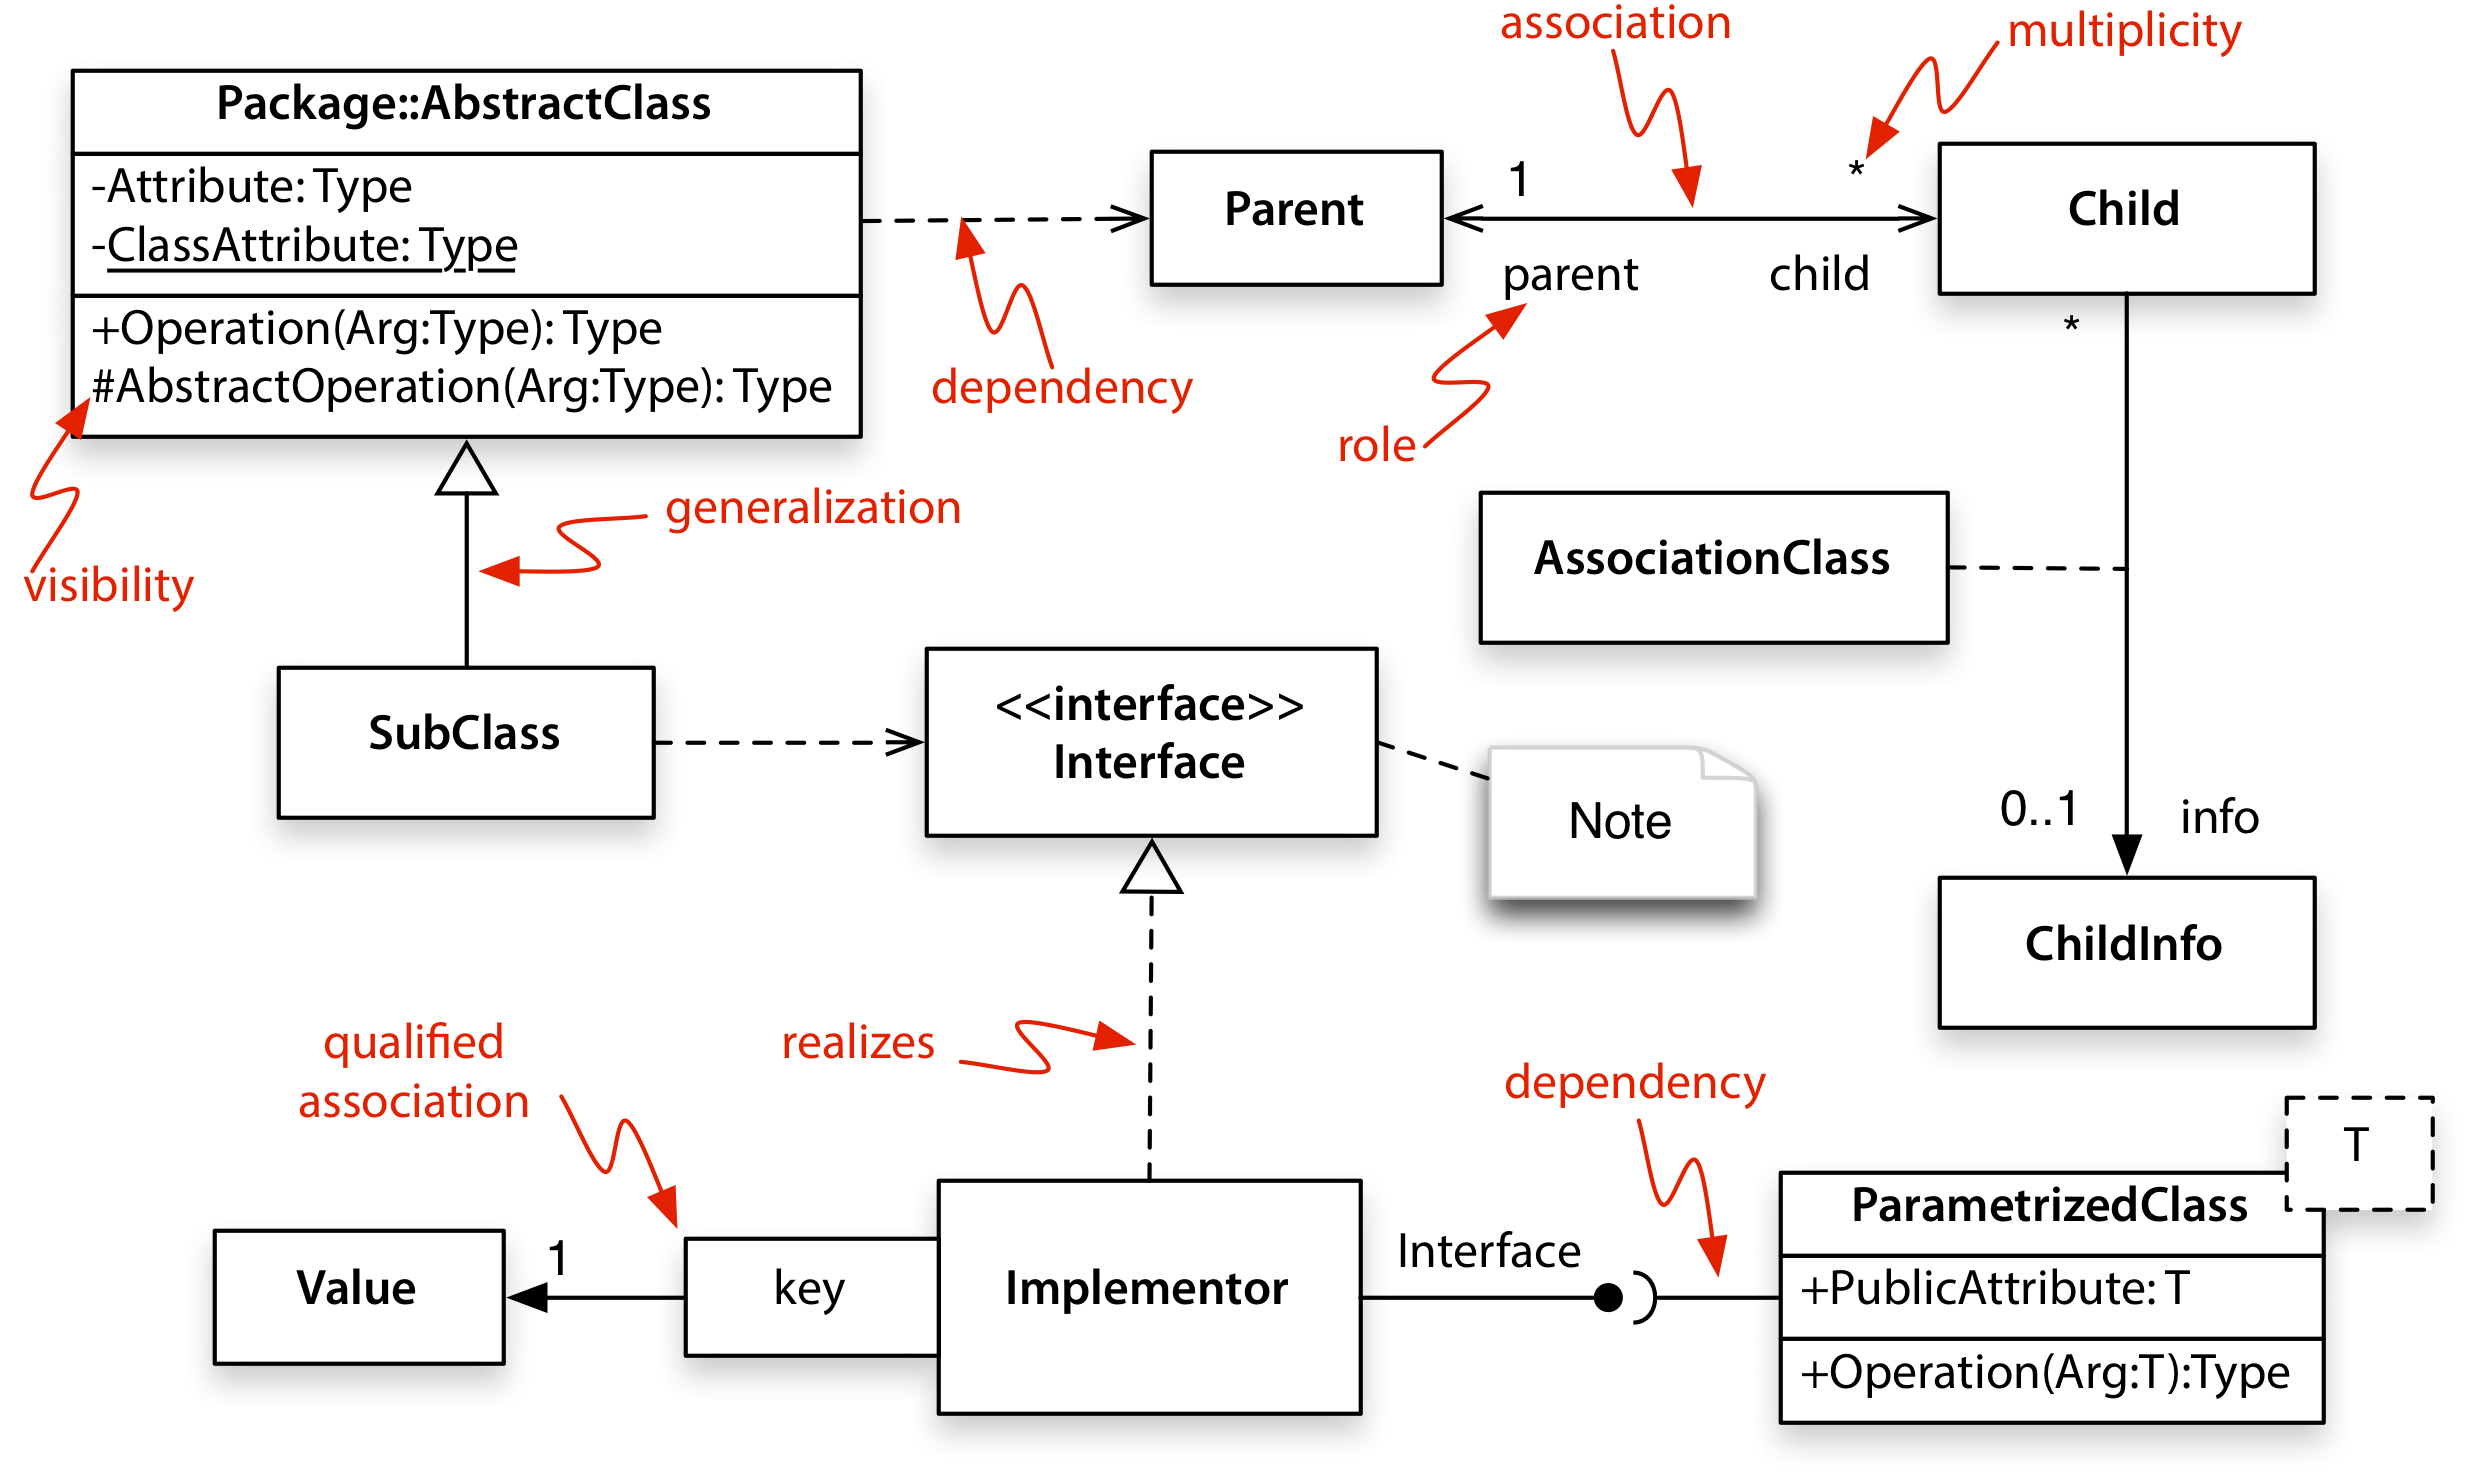
\includegraphics[height=180pt]{umlclasscheat.png}
\end{center}
  
\end{frame}

%--------
\begin{frame}{UML Overview}
The UML offers a rich set of diagram types to describe structure and behaviour.
    \begin{itemize}
       \item \textbf{\color{blue}Class diagrams} {\color{red}$\leftarrow$ this is what we use here}
      \item Component diagrams
       \item Activity diagrams {\color{red}$\leftarrow$ covered in "Real-Time Systems"}
       \item State charts  {\color{red}$\leftarrow$ covered in "Real-Time Systems"}
        \item Sequence diagrams
        \item Use case diagrams
         \item and eight more ...
   \end{itemize}
\end{frame}


%--------
\begin{frame}{Class Diagram: Overview}
    \begin{itemize}
       \item \Glspl{attribute} describe the appearance and knowledge of a class of objects.
       \item \Glspl{operation} define the behavior that a class of objects can manifest.
       \item \Glspl{stereotype} help you understand this type of object in the context of other classes 
                of objects with similar roles within the system’s design.
        \item \Glspl{property} provide a way to track the maintenance and status of the class definition.
        \item \Gls{association} is just a formal term for a type of relationship that this type of object may participate in. 
                 Associations may come in many variations, including simple, aggregate and composite, qualified, and reflexive.
         \item \Gls{inheritance} allows you to organize the class definitions to simplify and facilitate their implementation.
   \end{itemize}
\end{frame}

%--------
\begin{frame}{Class Diagram: Class Element Compartments}
\begin{center}
  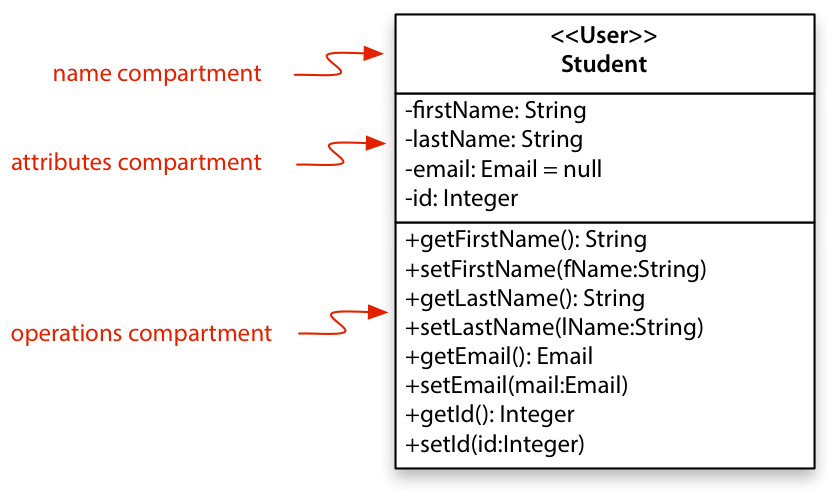
\includegraphics[height=180pt]{compartments.png}
\end{center}
  
\end{frame}

%-----------
\begin{frame}{Class Diagram:Modeling Attributes}{Attribute Visibility}
Each attribute definition must specify what other objects are allowed to see the attribute -- that is its visibility. 
Visibility is defined as follows:
    \begin{itemize}
         \item Public (+) visibility allows access to objects of all other classes.
         \item Private (-) visibility limits access to within the class itself. For example, only
operations of the class have access to a private attribute.
         \item Protected (\#) visibility allows access by subclasses. In the case of generalizations 
                   (inheritance), subclasses must have access to the attributes and operations of the superclass or 
                   they cannot be inherited.
         \item Package (\textasciitilde) visibility allows access to other objects in the same package.
   \end{itemize}
\end{frame}

%-----------
\begin{frame}{Class Diagram:Modeling Attributes}{Attribute Specification}

      \begin{tabular}{p{4.5cm}p{6.5cm}}
        \toprule
        \textbf{Attribute Element Description} & \textbf{Attribute Element Example}  \\
        \midrule
	\scriptsize Create an attribute name & \scriptsize company\\
	\scriptsize Add the attribute data type & \scriptsize company:character \\
	\scriptsize Add the attribute’s default value, if any & \scriptsize company:character = spaces \\
	\scriptsize Set the constraints on the attribute value. For this example, first identify the field length. &  
          \scriptsize         company:character = spaces \{1 to 30 characters\} \\
	\scriptsize Next identify the types of data that can be used in the attribute. Add this information within the brackets. & 
        \scriptsize    company:character = spaces \{1 to 30 characters including alphabetic, spaces, and punctuation 
                characters; no special characters allowed\} \\
	\scriptsize Set the attribute visibility (designate private visibility with a minus (-) sign in front of the attribute). 
        &\scriptsize  - company:character = spaces \{1 to 30 characters including alphabetic, spaces, and punctuation characters; 
                 no special characters allowed\} \\

        \bottomrule

      \end{tabular}
\end{frame}

%-----------
\begin{frame}{Class Diagram: Operations}
    \begin{itemize}
	\item Operation name: Required. The combination of name and parameters does need to be unique within a class.
	\item Arguments/parameters: Each argument requires an identifier and a data type. 
	\item Return data type: Required for a return value, but return values are optional. 
	\item Visibility (+, -, \#, \textasciitilde): Required before code generation. 
	\item Class level operation (underlined operation declaration): Optional. In Java: static methods.
	\item Argument name: Required for each parameter, but parameters are optional. Any number of arguments is allowed.
	\item Argument data type: Required for each parameter, but parameters are optional.
   \end{itemize}
\end{frame}

%--------
\begin{frame}{Class Diagram: Associations}
\begin{center}
  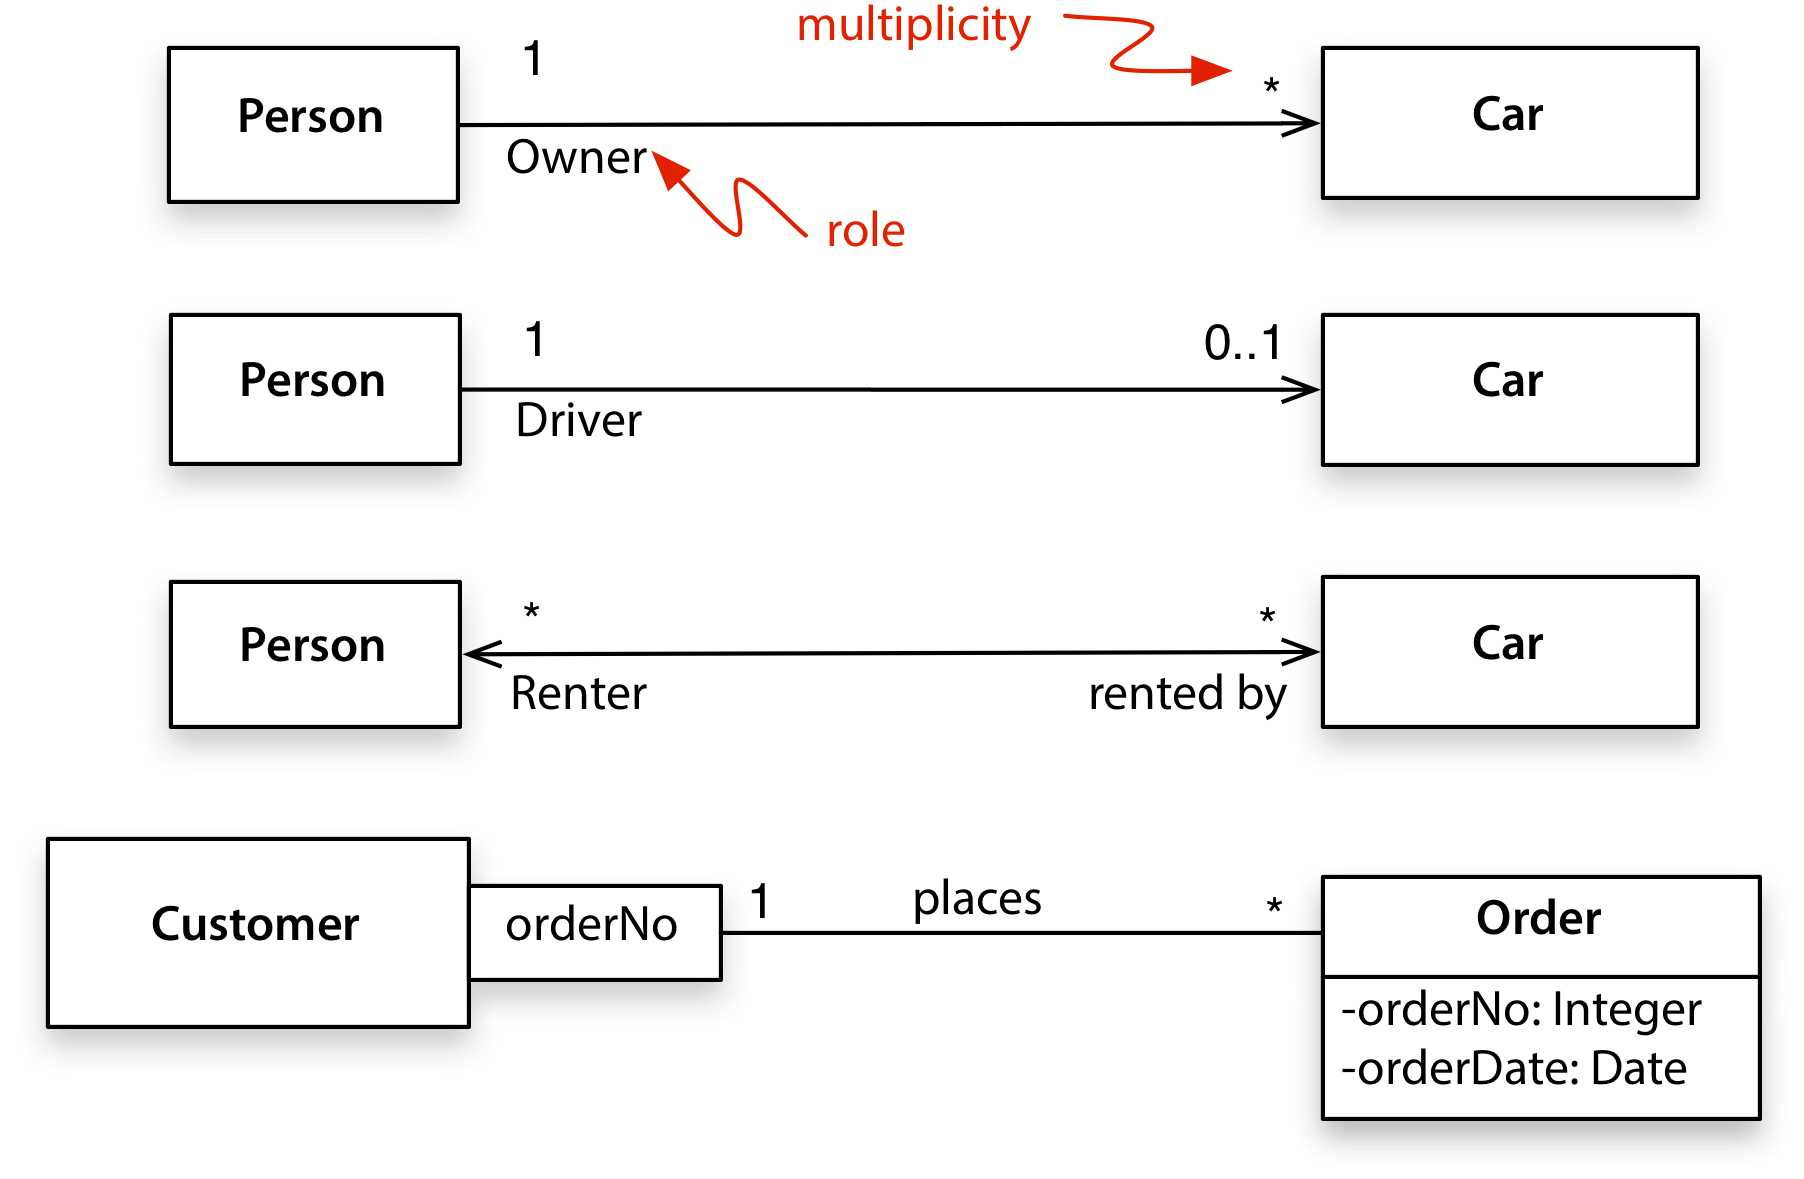
\includegraphics[scale=0.6]{associations.png}
\end{center}
  
\end{frame}

%--------
\begin{frame}{Class Diagram: Aggregation and Composition}
\begin{center}
  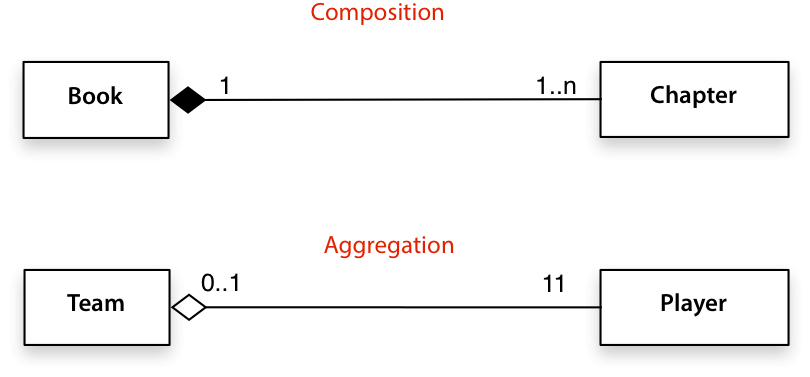
\includegraphics[scale=0.6]{aggregation.png}
\end{center}

\end{frame}

%--------
\begin{frame}{Class Diagram: Generalization}
\begin{center}
  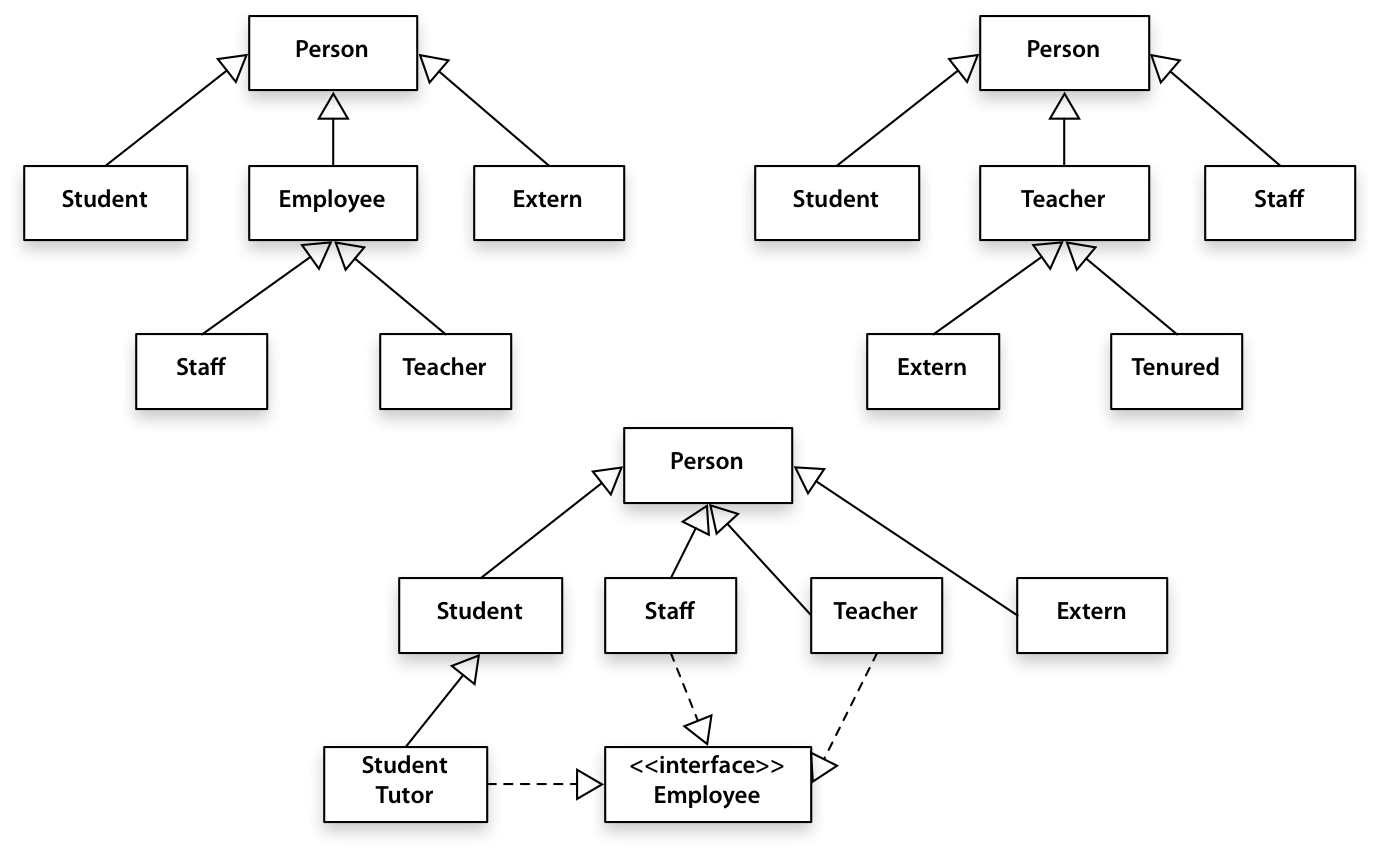
\includegraphics[height=190pt]{generalization.png}
\end{center}

\end{frame}

%***********************
% TODO more UML examples
%***********************
%
\begin{frame}{Architectural Objectives}
	The system to be designed must be
       \begin{itemize}
           \item correct
           \item extensible
           \item understandable
       \end{itemize}
	To that end we use object oriented design principles
\end{frame}

\begin{frame}{Principles of Object Oriented Design}
   \begin{block}{Principles for Single Class Design}
       \begin{itemize}
           \item Encapsulation, abstraction, and information hiding
           \item Separation of concerns and the single-responsibility principle
           \item Interface segregation principle
   \end{itemize}
   \end{block}
   \begin{block}{Principles for Design of Class Cooperation}
       \begin{itemize}
           \item Loose Coupling
           \item Liskov substitution principle
           \item Design by contract
           \item Open-close principle
           \item Dependency inversion principle
   \end{itemize}
\end{block}


\end{frame}

\subsection{Correctness, Extensibility, and Understandibility}
\subsubsection{Correctness}
\subsubsection{Extensibility}
\subsubsection{Understandibility}

\subsection{Encapsulation, abstraction, and information hiding}
\subsection{Separation of concerns and the single-responsibility principle}
\subsection{Interface segregation principle}
\subsection{Loose Coupling}
\subsection{Liskov substitution principle}
\subsection{Design by contract}
\subsection{Open-close principle}
\subsection{Dependency inversion principle}





\fi

\ifpartII
\section{Introduction}

\subsection{Die Dateien}

\begin{frame}[fragile]{Das Theme Esslingen für Beamer-Präsentationen}
Zum Paket gehören die folgenden Dateien:

\rowcolors{1}{HEblue4}{HEblue2}

\begin{center}
  \begin{tabular}{lp{6cm}}
    beamercolorthemeEsslingen.sty & Farbdefinitionen \\
    beamerfontthemeEsslingen.sty & Schriftauswahl \\
    beamerouterthemeEsslingen.sty & Kopf-, Fußzeile, Logo, Seitentitel\\
    beamerthemeEsslingen.sty & weitere Definitionen \\
    Esslingen-Defs.sty & die Farbdefinitionen zum Einbinden in \LaTeX-Dateien.\\
  \end{tabular}
\end{center}
Aufgerufen wird das Theme Esslingen in der Präambel mittels
\verb+\usetheme{Esslingen}+

\end{frame}

\begin{frame}{Abbildungen} 
Im Ordner \texttt{figures} befinden sich die folgenden Bilder im eps- und
png-Format sowie eine avi-Animation.

\rowcolors{1}{HEblue4}{HEblue2}
\begin{center}
  \begin{tabular}{lp{6cm}}
  HEGoeppingen & Das Hochschulgebäude \\
  HEGrid & Das Grid (Titelseite rechts oben) \\
  HELogo & Das Logo der Hochschule Esslingen \\
  TubeKnot & Das Standbild der Knoten-Animation \\
  TubeKnot.avi & Eine kurze Animation eines Knotens \\
  \end{tabular}
\end{center}

Die Bilder \texttt{HELogo}, \texttt{HEGoeppingen} und \texttt{HEGrid} werden
für die Titelseite benutzt. \texttt{HELogo} erscheint außerdem in jeder
Titelzeile eines Frames.

\end{frame}

\begin{frame}[fragile]{Die Beispiel-Datei}
Es liegt eine Beispiel-Datei in drei Formen bei. 
\rowcolors{1}{HEblue4}{HEblue2}
\begin{center}
  \begin{tabular}{lp{6cm}}
    example-beamer.tex &  die Beamer-Präsentation \\
    example-handout.tex & A4-Handout der Beamer-Frames \\
    example-article.tex & Article-Handout \\
  \end{tabular}
\end{center}

Die drei PDF-Dateien können entweder gemeinsam über das beiliegende make-File
oder einzeln mit den Befehlen
\begin{verbatim}
  pdflatex example-beamer.tex
  pdflatex example-handout.tex
  pdflatex example-article.tex
\end{verbatim}
erzeugt werden. Die drei LaTex-Dateien binden jeweils die Dateien
\texttt{preamble.tex} und \texttt{example.tex} ein.

\end{frame}

\section{Layout-Elemente}

\begin{frame}[fragile]{Die Fußzeile}
  \begin{itemize}
  \item Die Einträge in der Fußzeile werden aus den optionalen Argumenten der
  Befehle \texttt{title}, \texttt{subtitle}, \texttt{author},
  \texttt{\institute} und \texttt{date} in der Titelseite
  zusammengesetzt. 

  \item Die Fußzeile kann zwischen den Frames mit dem Befehl
\begin{verbatim}
   \setbeamertemplate{footline}{}
\end{verbatim}
für die nachfolgenden Frames ausgeschaltet werden. Dadurch gewinnt man etwas
Platz auf der Seite.
  \end{itemize}
\end{frame}

% Ausschalten der Fußzeile
\setbeamertemplate{footline}{}

\subsection{Die Farbtabelle}

\begin{frame}{Die Farbtabelle}
\label{frame:Farbtabelle}
\begin{table}[h]
    \centering
    \caption{Vordefinierte Farben entsprechend Corporate Design}
      \begin{tabular}{clll}
        \toprule
        \textbf{Farbe} & \textbf{Kürzel} & \textbf{RGB-Wert} & \textbf{Verwendungsbeispiel} \\
        \midrule
        \color{HEblue6}\rule{30pt}{8pt} & HEblue6 &    0,   70,  102 & Überschriften \\
        \color{HEblue5}\rule{30pt}{8pt} & HEblue5 &   85,  146,  172 &  \\
        \color{HEblue4}\rule{30pt}{8pt} & HEblue4 &  168,  203,  221 & Hauptüberschriften \\
        \color{HEblue3}\rule{30pt}{8pt} & HEblue3 &  206,  226,  236 &  \\
        \color{HEblue2}\rule{30pt}{8pt} & HEblue2 &  236,  242,  245 &  \\
        \color{HEblue1}\rule{30pt}{8pt} & HEblue1 &  245,  248,  249 & Abbildungshintergrund \\
        \color{HEgray1}\rule{30pt}{8pt} & HEgray1 &  112,  113,  114 & Aufzählungszeichen \\
        \color{HEred2}\rule{30pt}{8pt}  & HEred2  &  212,    0,   50 & Überschriften, Logo \\
        \color{HEred1}\rule{30pt}{8pt}  & HEred1  &  230,  143,  126 &  \\
        \bottomrule
      \end{tabular}
  \end{table}
\end{frame}

% 
\mode<article>{
\begin{figure}[h]
  \centering
  \fbox{\includeslide[height=5cm]{frame:Farbtabelle}}
  \caption{Bildimport aus der Präsentationsdatei.}
  \label{fig:slide.farbtabelle}
\end{figure}
}

\begin{frame}[fragile]{Die Fußzeile}
  Mit dem Befehl
\begin{verbatim}
  \setbeamertemplate{footline}[Esslingen theme]
\end{verbatim}
  wird die Fußzeile wieder auf die voreingestellte Variante zurückgesetzt.
\end{frame}

% Wiedereinschalten der Fußzeile
\setbeamertemplate{footline}[Esslingen theme]

\subsection{Listen}

\begin{frame}{Itemize-, Enumerate- und Description-Listen}

Die Itemize-Liste
    \begin{itemize}
      \item Erste Ebene.
       \begin{itemize}
        \item Zweite Ebene.
       \end{itemize}
    \end{itemize}

Die Enumerate-Liste
  \begin{enumerate}
   \item Erster Eintrag
    \begin{enumerate}
     \item Erster Eintrag, zweite Ebene
    \end{enumerate}
  \end{enumerate}

Die Description-Liste
  \begin{description}
  \item[Eintrag] Erläuterung
  \end{description}

\end{frame}

\begin{frame}{Anpassung der Listen-Items}
Das Layout der Zähler und Listen-Items lässt sich leicht anpassen. Diese
Möglichkeit sollte aber nur zurückhaltend genutzt werden.

\setbeamertemplate{itemize item}{\Large\guillemotright}
\setbeamertemplate{itemize subitem}{--}
\setbeamertemplate{itemize subsubitem}{\textbullet}

\begin{itemize}
   \item Erste Ebene.
       \begin{itemize}
        \item Zweite Ebene.
       \begin{itemize}
        \item Dritte Ebene.
       \end{itemize}
       \end{itemize}
\end{itemize}
\begin{enumerate}[1.]
  \item Erster Eintrag
  \begin{enumerate}[(i)]
  \item Erster Eintrag, zweite Ebene
  \begin{enumerate}[a)]
  \item Erster Eintrag, dritte Ebene
  \end{enumerate}
  \end{enumerate}
\end{enumerate}
\end{frame}

\subsection{Blöcke}

\begin{frame}[fragile]{Blöcke}
Ob die Blöcke mit farbigem Hintergrund ausgegeben werden und wie kräftig
dieser ist, kann mit den folgenden Color-Themes in der Datei preamble.text 
gesteuert werden. (Voreingestellt ist \texttt{rose}.)

  \begin{itemize}
  \item \begin{verbatim}% \usecolortheme{lily}% kein Farb-Hintergrund\end{verbatim}
  \item \begin{verbatim}\usecolortheme{rose}% dezenter Farb-Hintergrund\end{verbatim}
  \item \begin{verbatim}% \usecolortheme{orchid}% kräftiger Farb-Hintergrund\end{verbatim}
  \end{itemize}
  \begin{block}{Überschrift}
    Ein Block.
  \end{block}
  \begin{alertblock}{Überschrift}
    Ein Alert-Block.
  \end{alertblock}
  \begin{example}
    Ein Beispiel-Block.
  \end{example}
\end{frame}

\begin{frame}{Satz und Beweis}
  \begin{theorem}%[Ein Satz mit Namen]
    Lorem ipsum dolor sit amet, consetetur sadipscing elitr, sed diam nonumy
    eirmod tempor invidunt ut labore et dolore magna aliquyam erat, sed diam
    \begin{equation}
      \label{eq:Satz}
      \sum_{i=1}^{\infty}\frac{1}{x^2}
    \end{equation}
  \end{theorem}
  \begin{proof}%[Der Beweis eines benannten Satzes]
    Lorem ipsum dolor sit amet, consetetur sadipscing elitr, sed diam nonumy
    eirmod tempor invidunt ut labore et dolore magna aliquyam erat, sed diam
    voluptua. At vero eos et accusam et justo duo dolores et ea rebum. Stet
    clita kasd gubergren, no sea takimata sanctus est Lorem ipsum dolor sit
    amet. 
  \end{proof}
\end{frame}

\begin{frame}[fragile]{Listings}
Quellcode-Listings lassen sich in-line \lstinline|print "hello world"| und in
der lstlisting-Umgebung des Pakets listing.sty darstellen.

\begin{lstlisting}[frame=single, emph={cout}, emphstyle={\color{blue}}]
   cout << "Hello world!";
\end{lstlisting}
\end{frame}

\begin{frame}[fragile]{Java}
huuhu
\begin{lstlisting}[frame=single]
   import com.aurel.track;

 public class TestClass {
    private String dummy;
 }
   cout << "Hello world!";
\end{lstlisting}
\end{frame}

\subsection{Animationen}

\begin{frame}{Animationen}{Einbindung mit dem Paket multimedia.sty}
Wie und ob Animationen angezeigt werden, ist abhängig vom Betriebssystem und
vom PDF-Betrachter.

\begin{columns}
  \column{.5\textwidth}
Klicken Sie auf das Bild, um die Animation mit einem externen Betrachter anzuzeigen.
  \column{.45\textwidth}
  \movie[externalviewer]{
\includegraphics[scale=.5]{figures/TubeKnot}}{figures/TubeKnot.avi}
\end{columns}
\end{frame}




\begin{frame}{Zum Schluss}
  \begin{center}
    {\Huge \textcolor{HEblue6}{\bf Happy \LaTeX{}-ing!}}
  \end{center}
\end{frame}


\fi

\ifpartIII
\section{Introduction}

\subsection{Die Dateien}

\begin{frame}[fragile]{Das Theme Esslingen für Beamer-Präsentationen}
Zum Paket gehören die folgenden Dateien:

\rowcolors{1}{HEblue4}{HEblue2}

\begin{center}
  \begin{tabular}{lp{6cm}}
    beamercolorthemeEsslingen.sty & Farbdefinitionen \\
    beamerfontthemeEsslingen.sty & Schriftauswahl \\
    beamerouterthemeEsslingen.sty & Kopf-, Fußzeile, Logo, Seitentitel\\
    beamerthemeEsslingen.sty & weitere Definitionen \\
    Esslingen-Defs.sty & die Farbdefinitionen zum Einbinden in \LaTeX-Dateien.\\
  \end{tabular}
\end{center}
Aufgerufen wird das Theme Esslingen in der Präambel mittels
\verb+\usetheme{Esslingen}+

\end{frame}

\begin{frame}{Abbildungen} 
Im Ordner \texttt{figures} befinden sich die folgenden Bilder im eps- und
png-Format sowie eine avi-Animation.

\rowcolors{1}{HEblue4}{HEblue2}
\begin{center}
  \begin{tabular}{lp{6cm}}
  HEGoeppingen & Das Hochschulgebäude \\
  HEGrid & Das Grid (Titelseite rechts oben) \\
  HELogo & Das Logo der Hochschule Esslingen \\
  TubeKnot & Das Standbild der Knoten-Animation \\
  TubeKnot.avi & Eine kurze Animation eines Knotens \\
  \end{tabular}
\end{center}

Die Bilder \texttt{HELogo}, \texttt{HEGoeppingen} und \texttt{HEGrid} werden
für die Titelseite benutzt. \texttt{HELogo} erscheint außerdem in jeder
Titelzeile eines Frames.

\end{frame}

\begin{frame}[fragile]{Die Beispiel-Datei}
Es liegt eine Beispiel-Datei in drei Formen bei. 
\rowcolors{1}{HEblue4}{HEblue2}
\begin{center}
  \begin{tabular}{lp{6cm}}
    example-beamer.tex &  die Beamer-Präsentation \\
    example-handout.tex & A4-Handout der Beamer-Frames \\
    example-article.tex & Article-Handout \\
  \end{tabular}
\end{center}

Die drei PDF-Dateien können entweder gemeinsam über das beiliegende make-File
oder einzeln mit den Befehlen
\begin{verbatim}
  pdflatex example-beamer.tex
  pdflatex example-handout.tex
  pdflatex example-article.tex
\end{verbatim}
erzeugt werden. Die drei LaTex-Dateien binden jeweils die Dateien
\texttt{preamble.tex} und \texttt{example.tex} ein.

\end{frame}

\section{Layout-Elemente}

\begin{frame}[fragile]{Die Fußzeile}
  \begin{itemize}
  \item Die Einträge in der Fußzeile werden aus den optionalen Argumenten der
  Befehle \texttt{title}, \texttt{subtitle}, \texttt{author},
  \texttt{\institute} und \texttt{date} in der Titelseite
  zusammengesetzt. 

  \item Die Fußzeile kann zwischen den Frames mit dem Befehl
\begin{verbatim}
   \setbeamertemplate{footline}{}
\end{verbatim}
für die nachfolgenden Frames ausgeschaltet werden. Dadurch gewinnt man etwas
Platz auf der Seite.
  \end{itemize}
\end{frame}

% Ausschalten der Fußzeile
\setbeamertemplate{footline}{}

\subsection{Die Farbtabelle}

\begin{frame}{Die Farbtabelle}
\label{frame:Farbtabelle}
\begin{table}[h]
    \centering
    \caption{Vordefinierte Farben entsprechend Corporate Design}
      \begin{tabular}{clll}
        \toprule
        \textbf{Farbe} & \textbf{Kürzel} & \textbf{RGB-Wert} & \textbf{Verwendungsbeispiel} \\
        \midrule
        \color{HEblue6}\rule{30pt}{8pt} & HEblue6 &    0,   70,  102 & Überschriften \\
        \color{HEblue5}\rule{30pt}{8pt} & HEblue5 &   85,  146,  172 &  \\
        \color{HEblue4}\rule{30pt}{8pt} & HEblue4 &  168,  203,  221 & Hauptüberschriften \\
        \color{HEblue3}\rule{30pt}{8pt} & HEblue3 &  206,  226,  236 &  \\
        \color{HEblue2}\rule{30pt}{8pt} & HEblue2 &  236,  242,  245 &  \\
        \color{HEblue1}\rule{30pt}{8pt} & HEblue1 &  245,  248,  249 & Abbildungshintergrund \\
        \color{HEgray1}\rule{30pt}{8pt} & HEgray1 &  112,  113,  114 & Aufzählungszeichen \\
        \color{HEred2}\rule{30pt}{8pt}  & HEred2  &  212,    0,   50 & Überschriften, Logo \\
        \color{HEred1}\rule{30pt}{8pt}  & HEred1  &  230,  143,  126 &  \\
        \bottomrule
      \end{tabular}
  \end{table}
\end{frame}

% 
\mode<article>{
\begin{figure}[h]
  \centering
  \fbox{\includeslide[height=5cm]{frame:Farbtabelle}}
  \caption{Bildimport aus der Präsentationsdatei.}
  \label{fig:slide.farbtabelle}
\end{figure}
}

\begin{frame}[fragile]{Die Fußzeile}
  Mit dem Befehl
\begin{verbatim}
  \setbeamertemplate{footline}[Esslingen theme]
\end{verbatim}
  wird die Fußzeile wieder auf die voreingestellte Variante zurückgesetzt.
\end{frame}

% Wiedereinschalten der Fußzeile
\setbeamertemplate{footline}[Esslingen theme]

\subsection{Listen}

\begin{frame}{Itemize-, Enumerate- und Description-Listen}

Die Itemize-Liste
    \begin{itemize}
      \item Erste Ebene.
       \begin{itemize}
        \item Zweite Ebene.
       \end{itemize}
    \end{itemize}

Die Enumerate-Liste
  \begin{enumerate}
   \item Erster Eintrag
    \begin{enumerate}
     \item Erster Eintrag, zweite Ebene
    \end{enumerate}
  \end{enumerate}

Die Description-Liste
  \begin{description}
  \item[Eintrag] Erläuterung
  \end{description}

\end{frame}

\begin{frame}{Anpassung der Listen-Items}
Das Layout der Zähler und Listen-Items lässt sich leicht anpassen. Diese
Möglichkeit sollte aber nur zurückhaltend genutzt werden.

\setbeamertemplate{itemize item}{\Large\guillemotright}
\setbeamertemplate{itemize subitem}{--}
\setbeamertemplate{itemize subsubitem}{\textbullet}

\begin{itemize}
   \item Erste Ebene.
       \begin{itemize}
        \item Zweite Ebene.
       \begin{itemize}
        \item Dritte Ebene.
       \end{itemize}
       \end{itemize}
\end{itemize}
\begin{enumerate}[1.]
  \item Erster Eintrag
  \begin{enumerate}[(i)]
  \item Erster Eintrag, zweite Ebene
  \begin{enumerate}[a)]
  \item Erster Eintrag, dritte Ebene
  \end{enumerate}
  \end{enumerate}
\end{enumerate}
\end{frame}

\subsection{Blöcke}

\begin{frame}[fragile]{Blöcke}
Ob die Blöcke mit farbigem Hintergrund ausgegeben werden und wie kräftig
dieser ist, kann mit den folgenden Color-Themes in der Datei preamble.text 
gesteuert werden. (Voreingestellt ist \texttt{rose}.)

  \begin{itemize}
  \item \begin{verbatim}% \usecolortheme{lily}% kein Farb-Hintergrund\end{verbatim}
  \item \begin{verbatim}\usecolortheme{rose}% dezenter Farb-Hintergrund\end{verbatim}
  \item \begin{verbatim}% \usecolortheme{orchid}% kräftiger Farb-Hintergrund\end{verbatim}
  \end{itemize}
  \begin{block}{Überschrift}
    Ein Block.
  \end{block}
  \begin{alertblock}{Überschrift}
    Ein Alert-Block.
  \end{alertblock}
  \begin{example}
    Ein Beispiel-Block.
  \end{example}
\end{frame}

\begin{frame}{Satz und Beweis}
  \begin{theorem}%[Ein Satz mit Namen]
    Lorem ipsum dolor sit amet, consetetur sadipscing elitr, sed diam nonumy
    eirmod tempor invidunt ut labore et dolore magna aliquyam erat, sed diam
    \begin{equation}
      \label{eq:Satz}
      \sum_{i=1}^{\infty}\frac{1}{x^2}
    \end{equation}
  \end{theorem}
  \begin{proof}%[Der Beweis eines benannten Satzes]
    Lorem ipsum dolor sit amet, consetetur sadipscing elitr, sed diam nonumy
    eirmod tempor invidunt ut labore et dolore magna aliquyam erat, sed diam
    voluptua. At vero eos et accusam et justo duo dolores et ea rebum. Stet
    clita kasd gubergren, no sea takimata sanctus est Lorem ipsum dolor sit
    amet. 
  \end{proof}
\end{frame}

\begin{frame}[fragile]{Listings}
Quellcode-Listings lassen sich in-line \lstinline|print "hello world"| und in
der lstlisting-Umgebung des Pakets listing.sty darstellen.

\begin{lstlisting}[frame=single, emph={cout}, emphstyle={\color{blue}}]
   cout << "Hello world!";
\end{lstlisting}
\end{frame}

\begin{frame}[fragile]{Java}
huuhu
\begin{lstlisting}[frame=single]
   import com.aurel.track;

 public class TestClass {
    private String dummy;
 }
   cout << "Hello world!";
\end{lstlisting}
\end{frame}

\subsection{Animationen}

\begin{frame}{Animationen}{Einbindung mit dem Paket multimedia.sty}
Wie und ob Animationen angezeigt werden, ist abhängig vom Betriebssystem und
vom PDF-Betrachter.

\begin{columns}
  \column{.5\textwidth}
Klicken Sie auf das Bild, um die Animation mit einem externen Betrachter anzuzeigen.
  \column{.45\textwidth}
  \movie[externalviewer]{
\includegraphics[scale=.5]{figures/TubeKnot}}{figures/TubeKnot.avi}
\end{columns}
\end{frame}




\begin{frame}{Zum Schluss}
  \begin{center}
    {\Huge \textcolor{HEblue6}{\bf Happy \LaTeX{}-ing!}}
  \end{center}
\end{frame}


\fi

\printglossaries

\end{document}
